\section{Introduction}
\begin{frame}{\VideoName}
    \tableofcontents[currentsection]
\end{frame}

\begin{frame}{Countermeasures}
    \begin{itemize}
        \item Protocol level
        \begin{itemize}
            \item Design the usage of cryptographic primitives in a way that certain fault attacks are not possible anymore
            \item Re-keying\footnote{Medwed, M., Standaert, F. X., Großschädl, J., \& Regazzoni, F. (2010, May). Fresh re-keying: Security against side-channel and fault attacks for low-cost devices. In International Conference on Cryptology in Africa (pp. 279-296). Springer, Berlin, Heidelberg.}
        \end{itemize}
        \item Cryptographic primitive level
        \begin{itemize}
            \item Proposal of new cipher design\footnote{Baksi, A., Bhasin, S., Breier, J., Khairallah, M., Peyrin, T., Sarkar, S., \& Sim, S. M. (2021, December). DEFAULT: Cipher Level Resistance Against Differential Fault Attack. In International Conference on the Theory and Application of Cryptology and Information Security (pp. 124-156). Springer, Cham.}
        \end{itemize}
        \item Implementation level
        \begin{itemize}
            \item Infective countermeasure
            \item Redundancy
            \begin{itemize}
                \item Repeat the computation, e.g. deploy the circuit more than once
                \item \textcolor{blue}{Using error detecting/correcting codes}
            \end{itemize}
        \end{itemize}
            \end{itemize}
\end{frame}

\begin{frame}{Countermeasures}
    \begin{itemize}
        \item Hardware level
        \begin{itemize}
            \item Light sensors to detect the opening of chip
            \item Voltage/temperature sensors to detect fault injections by voltage glitches or temperature variations\footnote{Hutter, M., \& Schmidt, J. M. (2013, November). The temperature side channel and heating fault attacks. In International Conference on Smart Card Research and Advanced Applications (pp. 219-235). Springer, Cham.}
            \item On the other hand, there are new ways to induce faults proposed all the time. The main focus in academics is more on countermeasures that aim at managing the effect of fault induction.
        \end{itemize}
    \end{itemize}
\end{frame}


\begin{frame}{Binary code}
    \begin{definition}
\begin{itemize}
        \item $\boldsymbol{w}=w_0w_1\dots w_{n-1}\in\FF_2^n$ is called a \textit{binary word of length $n$}.
        \item A nonempty set $C\subset\FF_2^n$ is called a \textit{binary code}\index{binary code} of \textit{length}\index{binary code!length} $n$.
        \item An element of a binary code $C$ is called a \textit{codeword}\index{binary code!codeword} in $C$.
        \item Cardinality of $C$ is called the \textit{size}\index{binary code!size} of $C$.
        \item A code of length $n$ and size $M$ is called a \textit{binary $(n,M)-$code}\index{binary code!binary $(n,M)-$code}.
\end{itemize}
\end{definition}
\begin{example}
    \begin{itemize}
        \item $C=\Set{00,11}$ is a binary $(2,2)-$code.
        \item $C=\Set{010,001,110,111}$ is a binary $(3,4)-$code.
    \end{itemize}
\end{example}
\end{frame}


\begin{frame}{Encoding and decoding}
    \begin{itemize}
        \item Let us consider binary $(n,M)-$codes with $M=2^k$ for some positive integer $k$.
       \item When a binary code is used for transmitting information, every information word $\boldsymbol{u}\in\FF_2^k$ is assigned a unique codeword $\boldsymbol{c}(\boldsymbol{u})\in C$.
       \item We say that $\boldsymbol{u}$ is \textit{encoded} as $\boldsymbol{c}(\boldsymbol{u})$.
       \item Suppose Alice would like to send information $\boldsymbol{u}$ to Bob using $C$.
       \item Alice sends codeword $\boldsymbol{c}(\boldsymbol{u})$ to Bob.
        \item Due to transmission noise, Bob might receive a word $\boldsymbol{x}\in\FF_2^n$ not equal to $\boldsymbol{c}(\boldsymbol{u})$.
       \item Thus we need to define a \textit{decoding rule} for Bob that allows him to find $\boldsymbol{u}$ given $\boldsymbol{x}$.
       \item For our countermeasure, our decoding rule is as follows:
       \begin{itemize}
           \item output an error message if the received word is not a codeword
           \item otherwise, we decode it to the corresponding information
       \end{itemize}
    \end{itemize}
\end{frame}

\begin{frame}{Encoding and decoding -- Example}
    \begin{example}
    \begin{itemize}
        \item Let $C=\Set{0000,0111, 1110, 1111}$.
         \item We use $C$ to encode information words $\boldsymbol{u}\in\FF_2^2$ with encoding designed as follows:
\[
c(00)=0000,\quad c(01)=0111,\quad c(10)=1110,\quad c(11)=1111.
\]
\item Suppose Alice sends information $00$ with codeword $0000$ to Bob.
\item Due to an error during the transmission, Bob receives $0001$.
\item Our decoding rule outputs an error
\item If Bob receives $0111$, then he decodes it to $01$, and gets a wrong message
    \end{itemize}
\end{example}
\begin{alertblock}{Remark}
    We can see that when the received word is not a codeword, we can \textit{detect} there is an error, or bit flip.
    Thus, we also refer to binary code as \textit{error-detecting} code.
\end{alertblock}
\end{frame}


\section{Encoding-based Countermeasure for PRESENT}
\begin{frame}{\VideoName}
    \tableofcontents[currentsection]
\end{frame}

\begin{frame}{Error-detecting code as countermeasure}
    \begin{itemize}
        \item A binary code can detect bit flips
        \item A natural choice for fault countermeasure is to consider encoding the intermediate values during the computation.
        \item Which code to choose and how to implement it?
        \item We will discuss one proposal of using binary code for the countermeasure against bit flips and instruction skips\footnote{Breier, J., Hou, X., \& Liu, Y. (2019). On evaluating fault resilient encoding schemes in software. IEEE Transactions on Dependable and Secure Computing, 18(3), 1065-1079.}.
        \item See the original paper for
        \begin{itemize}
            \item Formalization of encoding-based countermeasure for symmetric block ciphers
           \item Calculation of the probability for detecting any $m-$bit flip and for instruction skips
        \end{itemize}
    \end{itemize}
\end{frame}


\begin{frame}{Encoding countermeasure for PRESENT}
\begin{itemize}
    \item Each operation is implemented as a lookup table from memory.
    \item Before the table lookup, the destination register of an operation is precharged to $\boldsymbol{0}$.
    \item When any of the inputs is $\boldsymbol{0}$, the output is $\boldsymbol{0}$.
    \item When an error is detected, the output is $\boldsymbol{0}$ (error message).
    \item We assume the registers are precharged to $\boldsymbol{0}$ before the program starts and this process cannot be faulted.
\end{itemize}
Such a design can protect the implementation from single instruction skips -- e.g. A single instruction skip of any instruction of the following algorithm will either make no change to the output or result in outputting $\boldsymbol{0}$ (error message).
{
\setlength{\interspacetitleruled}{0pt}%
\setlength{\algotitleheightrule}{0pt}%
\begin{algorithm}[H]
	\texttt{LDI r0 a}\tcp{load input a}
\texttt{LDI r1 b}\tcp{load input b}
	\texttt{EOR r2 r2}\tcp{precharge register \texttt{r2} to zero}
	\texttt{LPM r2 r0 r1}\tcp{execution of an operation by table lookup}
\end{algorithm}
}
\end{frame}

\begin{frame}{Error message cannot be a codeword}
    \begin{itemize}
        \item Do not contain $\boldsymbol{0}$ as a codeword.
        \item Of course, the error message can be changed to a different value as long as it is not a codeword and has the same bit length as the codewords
    \end{itemize}
\end{frame}

\begin{frame}{Detected and undetected faults}
    \begin{itemize}
        \item In case the fault changes some encoded intermediate value to a word that is not a codeword, the table lookup will produce $\boldsymbol{0}$, which indicates an error.
        \item In the subsequent instructions, when the input of a table is $\boldsymbol{0}$, the output will always be $\boldsymbol{0}$ since $\boldsymbol{0}$ is not a codeword.
         \item In such cases, we say that the fault is \textit{detected}.
        \item Otherwise, when a successful fault injection does not result in $\boldsymbol{0}$ output, we say the fault is \textit{undetected}.
    \end{itemize}
\end{frame}


\begin{frame}{Lookup table for an operation -- Example}
    \begin{example}
    \begin{itemize}
        \item As a simple example, let us consider $\Set{01,10}$, a binary $(2,2)-$code.
        \item Since there are two codewords, it can be used to encode one bit of information.
        \item Let $0\mapsto 01$, $1\mapsto 10$
        \item The lookup table for carrying out \texttt{XOR} between $a,b$ ($a,b\in\FF_2$) is shown in the following table.
        \item The table outputs $00$ (error message) if one input is not a codeword
    \end{itemize}
\begin{table}[htb]
    \centering
    \begin{tabular}{c|c|c|c|c}
          &  00  &  01  & 10  & 11\\\hline
      00  &  00  &  00  & 00  & 00\\
      01  &  00  &  01  & 10   & 00 \\
      10  &  00  &  10  & 01  & 00 \\
      11  &  00  &  00  & 00  & 00 
    \end{tabular}
\end{table}
\end{example}
\end{frame}

\begin{frame}{Fault in the inputs -- Example}
    \begin{example}
        \begin{table}[htb]
    \centering
    \begin{tabular}{c|c|c|c|c}
          &  00  &  01  & 10  & 11\\\hline
      00  &  00  &  00  & 00  & 00\\
      01  &  00  &  01  & 10   & 00 \\
      10  &  00  &  10  & 01  & 00 \\
      11  &  00  &  00  & 00  & 00 
    \end{tabular}
\end{table}
\begin{itemize}
    \item $1-$bit flip will be detected:
    \begin{itemize}
        \item If $1-$bit flip is injected in input $01$, we get either $00$ or $11$, both will give output $00$.
        \item If $1-$bit flip is injected in input $10$, we will have $00$ or $11$ and output will again be $00$.
    \end{itemize}
    \item A $2-$bit flip will be undetected.
    \begin{itemize}
        \item Suppose we would like to compute $0\oplus 0$
        \item Inputs for the table lookup will be $01$ and $01$, the output will be $01$
        \item If a $2-$bit flip is injected in one of the inputs, we get $10$ and $01$ for table lookup and the result will be $10$
    \end{itemize}
\end{itemize}
    \end{example}
\end{frame}

\begin{frame}{PRESENT}
    \begin{itemize}
        \item Proposed in 2007 as a symmetric block cipher optimized for hardware implementation.
       \item block length: $64$
       \item number of rounds: $31$
       \item key length: either $80$ or $128$.
    \end{itemize}
\end{frame}

\begin{frame}{PRESENT -- encryption}
\begin{columns}[T] % align columns
\begin{column}{.55\textwidth}
\begin{itemize}
    \item Round function: addRoundKey, sBoxLayer, and pLayer.
    \item After $31$ rounds, addRoundKey is applied again before the ciphertext output 
\end{itemize}
\begin{alertblock}{Remark}
    For PRESENT specification, we consider the $0$th bit of a value as the rightmost bit in its binary representation.
For example, the $0$th bit of $3=011_2$ is $1$, the $1$st bit is $1$ and the $2$nd bit is $0$.
\end{alertblock}
\end{column}%
\hfill%
\begin{column}{.5\textwidth}
\begin{figure}
    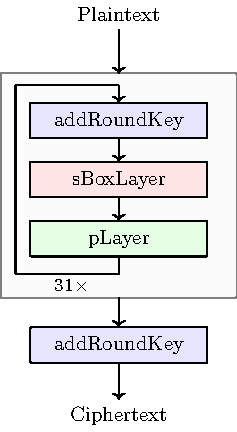
\includegraphics[width=0.6\textwidth]{fig/PRESENT.pdf}
\end{figure}
\end{column}%
\end{columns}
\end{frame}

\begin{frame}{PRESENT -- addRoundKey}
    \begin{itemize}
        \item Round key $K_i=\kappa^i_{63}\dots\kappa_0^i$, $(1\leq i\leq 32)$
        \item Current state $b_{63}b_{62}\dots b_0$
        \item For $0\leq j\leq 63$
    \end{itemize}
    \[
b_j\to b_j\oplus\kappa_j^i
\]
\end{frame}

\begin{frame}{PRESENT -- sBoxLayer}
    \begin{itemize}
        \item sBoxLayer applies sixteen $4-$bit Sboxes to each nibble of the current cipher state.
        \item For example, if the input is \texttt{0}, the output is \texttt{C}.
\begin{table}[htb]
\centering
\ttfamily
\begin{tabular}{cccccccccccccccc}\hline
 0 & 1 & 2 & 3 & 4 & 5 & 6 & 7 & 8 & 9 & A & B & C & D & E & F \\\hline
 C & 5 & 6 & B & 9 & 0 & A & D & 3 & E & F & 8 & 4 & 7 & 1 & 2\\\hline
\end{tabular}
\end{table}
    \end{itemize}
\begin{figure}
    \centering
    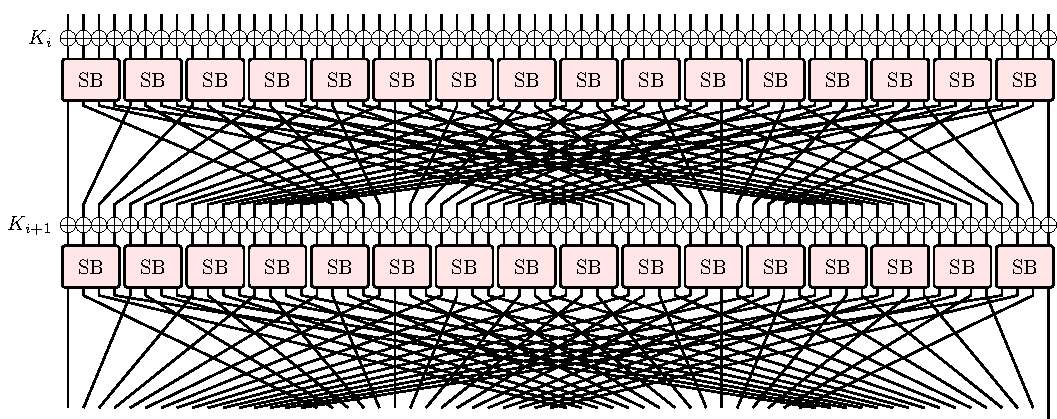
\includegraphics[width=0.9\textwidth]{fig/PRESENT_two_rounds.pdf}
\end{figure}
\end{frame}


\begin{frame}{PRESENT -- pLayer}
pLayer permutes the $64$ bits using the following formula:
\[
\text{pLayer}(j)=\left\lfloor\frac{j}{4}\right\rfloor+(j\mo 4)\times16,
\]
where $j$ denotes the bit position.
\begin{table}[htb]
\centering
\begin{tabular}{cccccccccccccccc}\hline
0 & 1 & 2 & 3 & 4 & 5 & 6 & 7 & 8 & 9 & 10 & 11 & 12 & 13 & 14 & 15 \\
0 & 16 & 32 & 48 & 1 & 17 & 33 & 49 & 2 & 18 & 34 & 50 & 3 & 19 & 35 & 51 \\\hline
16 & 17 & 18 & 19 & 20 & 21 & 22 & 23 & 24 & 25 & 26 & 27 & 28 & 29 & 30 & 31 \\
4 & 20 & 36 & 52 & 5 & 21 & 37 & 53 & 6 & 22 & 38 & 54 & 7 & 23 & 39 & 55 \\\hline
32 & 33 & 34 & 35 & 36 & 37 & 38 & 39 & 40 & 41 & 42 & 43 & 44 & 45 & 46 & 47 \\
8 & 24 & 40 & 56 & 9 & 25 & 41 & 57 & 10 & 26 & 42 & 58 & 11 & 27 & 43 & 59 \\\hline
48 & 49 & 50 & 51 & 52 & 53 & 54 & 55 & 56 & 57 & 58 & 59 & 60 & 61 & 62 & 63 \\
12 & 28 & 44 & 60 & 13 & 29 & 45 & 61 & 14 & 30 & 46 & 62 & 15 & 31 & 47 & 63\\\hline
\end{tabular}
\end{table}
\end{frame}

\begin{frame}{Quotient group and Remainder group}
    \begin{itemize}
        \item Before we go into details of the countermeasure implementation, we introduce the notion of Quotient group and Remainder group.
        \item We number the Sboxes in the $i$th round of PRESENT as $\text{SB}^i_0, \text{SB}^i_1,\dots,\text{SB}^i_{15}$, where $\text{SB}^i_0$ is the right most Sbox
       \item Those Sboxes can be grouped in $2$ different ways: the \textit{Quotient group} and the \textit{Remainder group}:
\[
    Qj^i:=\Set{\text{SB}^i_{4j},\text{SB}^i_{4j+1},\text{SB}^i_{4j+2},\text{SB}^i_{4j+3}},\quad Rj^i:=\Set{\text{SB}^i_{j},\text{SB}^i_{j+4},\text{SB}^i_{j+8},\text{SB}^i_{j+12}},
\]
where $j=0,1,2,3$.
\item Such a grouping allows us to relate the bits for each Sbox output in round $i$ to bits of each Sbox input in round $i+1$ in a certain way through pLayer
    \end{itemize}
\end{frame}

\begin{frame}{Quotient group and Remainder group}
    \begin{table}[H]
        \centering
        \begin{tabular}{|c|c|c|c|c|}\hline
                \backslashbox{$Rj^{i+1}$}{$Qj^i$}          &  $\text{SB}^i_{4j}$ & $\text{SB}^i_{4j+1}$ & $\text{SB}^i_{4j+2}$ & $\text{SB}^i_{4j+3}$\\\hline
        $\text{SB}^{i+1}_{j}$    &  $(0,0)$     &    $(1,0)$    &   $(2,0)$     &   $(3,0)$    \\\hline
        $\text{SB}^{i+1}_{j+4}$  &  $(0,1)$     &    $(1,1)$    &   $(2,1)$     &   $(3,1)$    \\\hline
        $\text{SB}^{i+1}_{j+8}$  &  $(0,2)$     &    $(1,2)$    &   $(2,2)$     &   $(3,2)$    \\\hline
        $\text{SB}^{i+1}_{j+12}$ &  $(0,3)$     &    $(1,3)$    &   $(2,3)$     &   $(3,3)$    \\\hline
        \end{tabular}
        \caption{Relation between the output bits of Sboxes from the Quotient group $Qj^i$ and the input bits of Sboxes from the corresponding Remainder group $Rj^{i+1}$.
        For example, the $0$th input bit of SB$_{j+4}^{i+1}$ in $Rj^{i+1}$ comes from the $1$st output bit of $\text{SB}^i_{4j}$ in $Qj^i$..}
\end{table}
\begin{itemize}
    \item Bits of the $0$th Sbox ($\text{SB}^i_{4j}$) output in Quotient group $Qj^i$ are permuted to the $0$th bits of Sbox inputs in the corresponding Remainder group $Rj^{i+1}$;
    \item Bits of the $1$st Sbox ($\text{SB}^i_{4j+1}$) output in $Qj^i$ are permuted to the $1$st bits of Sbox inputs in $Rj^{i+1}$;
\end{itemize}
\end{frame}

\begin{frame}{Quotient group and Remainder group}
    \begin{figure}[htb]
    \centering
    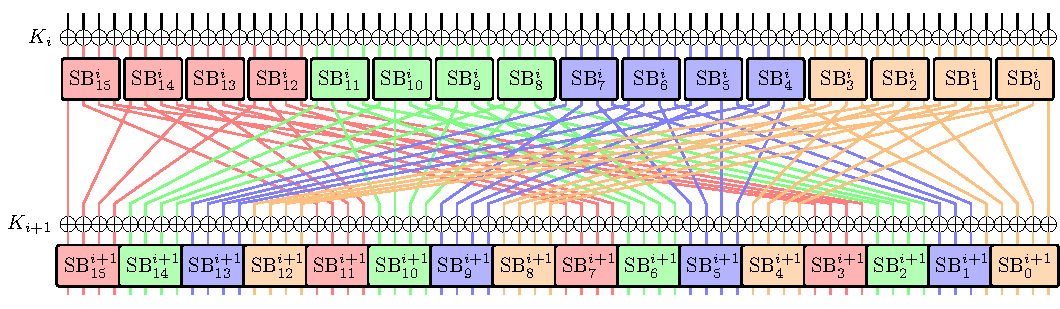
\includegraphics[width=1.0\textwidth]{fig/PRESENT_Sbox_grouping.pdf}
    \caption{An illustration of the relation between Sbox outputs in a Quotient group to Sbox inputs in the corresponding Remainder group.
    Sboxes in Quotient groups $Q0^i$, $Q1^i$, $Q2^i$, $Q3^i$ and their corresponding Remainder groups $R0^{i+1}$, $R1^{i+1}$, $R2^{i+1}$, $R3^{i+1}$ are in \textcolor{orange!50}{orange}, \textcolor{blue!50}{blue}, \textcolor{green!50}{green}, \textcolor{red!50}{red} colors respectively.}
\end{figure}
pLayer can be considered as four identical parallel bitwise operations where each is a function$:\FF_2^{16}\to\FF_2^{16}$ that takes one Quotient group output and permutes it to the corresponding Remainder group input.
\end{frame}

\begin{frame}{Choice of the binary code}
    \begin{itemize}
        \item pLayer can be considered as four identical parallel bitwise operations where each is a function$:\FF_2^{16}\to\FF_2^{16}$
        \item addRoundKey is a function$:\FF_2^{64}\to\FF_2^{64}$.
     \item Present Sbox SB$:\FF_2^{4}\to\FF_2^{4}$.
      \item One convenient code choice would be those with cardinalities $16$, encoding $4$ bits of information.
     \item In particular, we are looking for a binary $(n,16)-$code.
    \end{itemize}
\end{frame}

\begin{frame}{Choice of the binary code}
    \begin{itemize}
     \item See the original paper\footnote{Breier, J., Hou, X., \& Liu, Y. (2019). On evaluating fault resilient encoding schemes in software. IEEE Transactions on Dependable and Secure Computing, 18(3), 1065-1079.} for an algorithm for finding binary codes that achieve a low probability of undetected faults with certain given parameters.
     \item In the rest of this presentation, we will use the following binary $(8,16)-$code as a running example
\begin{equation*}
    \Set{\texttt{01, 08, 02, 0B, 04, 1D, 1E, 30, 7, 65, 6A, AD, B3, CE, D9, F6}}.
\end{equation*}
\item \texttt{01} is the codeword for $0000$, \texttt{08} in the codeword for $0001$, etc.
\item We write 
\[
\texttt{01}=\texttt{encode}(0000).
\]
    \end{itemize}
\end{frame}

\begin{frame}{Encoding countermeasure - addRoundKey}
    \begin{itemize}
        \item Given a binary code $C$, the addRoundKey operation can be implemented using an \texttt{XOR} table similar to the one we have seen before
        \item The size of the table will be $2^8\times2^8$.
        \item Let $\widetilde{\oplus}$ denote this table lookup operation.
    \end{itemize}
    \begin{example}[The previous example]
    \begin{itemize}
        \item $\Set{01,10}$, a binary $(2,2)-$code.
        \item $0\mapsto 01$, $1\mapsto 10$
        \item The lookup table for carrying out \texttt{XOR} between $a,b$ ($a,b\in\FF_2$) is shown in the following table.
    \end{itemize}
\begin{table}[htb]
    \centering
    \begin{tabular}{c|c|c|c|c}
          &  00  &  01  & 10  & 11\\\hline
      00  &  00  &  00  & 00  & 00\\
      01  &  00  &  01  & 10   & 00 \\
      10  &  00  &  10  & 01  & 00 \\
      11  &  00  &  00  & 00  & 00 
    \end{tabular}
\end{table}
\end{example}
\end{frame}

\begin{frame}{Encoding countermeasure - addRoundKey}
    \begin{itemize}
        \item Given a binary code $C$, the addRoundKey operation can be implemented using an \texttt{XOR} table similar to the one we have seen before
        \item The size of the table will be $2^8\times2^8$.
        \item Let $\widetilde{\oplus}$ denote this table lookup operation.
    \end{itemize}
\begin{example}
\begin{equation*}
    \Set{\texttt{01, 08, 02, 0B, 04, 1D, 1E, 30, 07, 65, 6A, AD, B3, CE, D9, F6}}.
\end{equation*}
The table entry corresponding to \texttt{01} and \texttt{08} will be
    \[
    \texttt{encode}(0000\oplus0001)=\texttt{encode}(0001)=\texttt{08}.
    \]
And we write
    \[
    \texttt{01}\widetilde{\oplus}\texttt{08}=\texttt{08}.
    \]
\end{example}
\end{frame}

\begin{frame}{Encoding countermeasure - sBoxLayer and pLayer}
\begin{itemize}
    \item The implementation of sBoxLayer and pLayer are based on four $16\times 64$ lookup tables, $T0, T1, T2,T3$.
    \item Let $\boldsymbol{x}=x_3x_2x_1x_0$ be an element in $\FF_2^4$.
    \item We write 
\[
\text{SB}(x_3x_2x_1x_0)=x^s_3x^s_2x^s_1x^s_0.
\]
\end{itemize}
\begin{table}[htb]
\centering
\ttfamily
\begin{tabular}{cccccccccccccccc}\hline
 0 & 1 & 2 & 3 & 4 & 5 & 6 & 7 & 8 & 9 & A & B & C & D & E & F \\\hline
 C & 5 & 6 & B & 9 & 0 & A & D & 3 & E & F & 8 & 4 & 7 & 1 & 2\\\hline
\end{tabular}
\end{table}
\begin{example}
    Take $\texttt{D}=1101$, then $x_3=1$, $x_2=1$, $x_1=0$, $x_0=1$.
    Since SB$(\texttt{D})=7=0111$, we have
    \[
    x_3^s=0,\ x_2^s=1,\ x_1^s=1,\ x_0^s=1.
    \]
\end{example}
\end{frame}


\begin{frame}{Encoding countermeasure - sBoxLayer and pLayer}
\begin{eqnarray*}
T0:C &\to& C\times C\times C\times C\\
\texttt{encode}(x_3x_2x_1x_0) &\mapsto& \texttt{encode}(000x^s_3),\texttt{encode}(000x^s_2),\texttt{encode}(000x^s_1),\texttt{encode}(000x^s_0)
\end{eqnarray*}
\begin{eqnarray*}
T1:C &\to& C\times C\times C\times C\\
\texttt{encode}(x_3x_2x_1x_0) &\mapsto& \texttt{encode}(00x^s_30),\texttt{encode}(00x^s_20),\texttt{encode}(00x^s_10),\texttt{encode}(00x^s_00)
\end{eqnarray*}
\begin{eqnarray*}
T2:C &\to& C\times C\times C\times C\\
\texttt{encode}(x_3x_2x_1x_0) &\mapsto& \texttt{encode}(0x^s_300),\texttt{encode}(0x^s_200),\texttt{encode}(0x^s_100),\texttt{encode}(0x^s_000)
\end{eqnarray*}
\begin{eqnarray*}
T3:C &\to& C\times C\times C\times C\\
\texttt{encode}(x_3x_2x_1x_0) &\mapsto& \texttt{encode}(x^s_3000),\texttt{encode}(x^s_2000),\texttt{encode}(x^s_1000),\texttt{encode}(x^s_0000)
\end{eqnarray*}
\end{frame}

\begin{frame}{Encoding countermeasure - sBoxLayer and pLayer}
\begin{itemize}
    \item Each table extracts the bits of Sbox output, permutes them and outputs the corresponding codeword.
    \item Each entry of the outputs of each table can be 
    \begin{itemize}
        \item $T0$: \texttt{encode}$(0000)$ or
\texttt{encode}$(0001)$
\item $T1$: \texttt{encode}$(0000)$ or
\texttt{encode}$(0010)$
\item $T2$: \texttt{encode}$(0000)$ or
\texttt{encode}$(0100)$
\item $T3$: \texttt{encode}$(0000)$ or
\texttt{encode}$(1000)$
    \end{itemize}
\end{itemize}

\end{frame}


\begin{frame}{Encoding countermeasure - sBoxLayer and pLayer}
\begin{eqnarray*}
T0:C &\to& C\times C\times C\times C\\
\texttt{encode}(x_3x_2x_1x_0) &\mapsto& \texttt{encode}(000x^s_3),\texttt{encode}(000x^s_2),\texttt{encode}(000x^s_1),\texttt{encode}(000x^s_0)
\end{eqnarray*}
    \begin{example}
    \begin{equation*}
    \Set{\texttt{01, 08, 02, 0B, 04, 1D, 1E, 30, 07, 65, 6A, AD, B3, CE, D9, F6}}.
\end{equation*}
\begin{itemize}
    \item Suppose the input is $\texttt{01}=\texttt{encode}(0000)$.
    \item The corresponding Sbox output would be $\texttt{C}=1100$, i.e. $x^s_3x^s_2x^s_1x^s_0=1100$.
    \item  The output of $T0$ will be 
     \begin{eqnarray*}
    &\texttt{encode}(0001)=\texttt{08}, 
    &\texttt{encode}(0001)=\texttt{08},\\
    &\texttt{encode}(0000)=\texttt{01},
    &\texttt{encode}(0000)=\texttt{01}.
     \end{eqnarray*}
\end{itemize}
\end{example}
\end{frame}


\begin{frame}{Encoding countermeasure - sBoxLayer and pLayer}
\begin{eqnarray*}
T1:C &\to& C\times C\times C\times C\\
\texttt{encode}(x_3x_2x_1x_0) &\mapsto& \texttt{encode}(00x^s_30),\texttt{encode}(00x^s_20),\texttt{encode}(00x^s_10),\texttt{encode}(00x^s_00)
\end{eqnarray*}
    \begin{example}
    \begin{equation*}
    \Set{\texttt{01, 08, 02, 0B, 04, 1D, 1E, 30, 07, 65, 6A, AD, B3, CE, D9, F6}}.
\end{equation*}
\begin{itemize}
    \item Suppose the input is $\texttt{01}=\texttt{encode}(0000)$.
    \item The corresponding Sbox output would be $\texttt{C}=1100$, i.e. $x^s_3x^s_2x^s_1x^s_0=1100$.
    \item  The output of $T1$ will be
    \begin{eqnarray*}
    &\texttt{encode}(0010)=\texttt{02}, 
    &\texttt{encode}(0010)=\texttt{02},\\ 
    &\texttt{encode}(0000)=\texttt{01},
    &\texttt{encode}(0000)=\texttt{01}.
    \end{eqnarray*}
\end{itemize}
\end{example}
\end{frame}

\begin{frame}{Encoding countermeasure - sBoxLayer and pLayer}
\begin{eqnarray*}
T2:C &\to& C\times C\times C\times C\\
\texttt{encode}(x_3x_2x_1x_0) &\mapsto& \texttt{encode}(0x^s_300),\texttt{encode}(0x^s_200),\texttt{encode}(0x^s_100),\texttt{encode}(0x^s_000)
\end{eqnarray*}
    \begin{example}
    \begin{equation*}
    \Set{\texttt{01, 08, 02, 0B, 04, 1D, 1E, 30, 07, 65, 6A, AD, B3, CE, D9, F6}}.
\end{equation*}
\begin{itemize}
    \item Suppose the input is $\texttt{01}=\texttt{encode}(0000)$.
    \item The corresponding Sbox output would be $\texttt{C}=1100$, i.e. $x^s_3x^s_2x^s_1x^s_0=1100$.
    \item  The output of $T2$ will be 
     \begin{eqnarray*}
     &\texttt{encode}(0100)=\texttt{04}, 
     &\texttt{encode}(0100)=\texttt{04},\\ 
     &\texttt{encode}(0000)=\texttt{01},
     &\texttt{encode}(0000)=\texttt{01}.
     \end{eqnarray*}
\end{itemize}
\end{example}
\end{frame}


\begin{frame}{Encoding countermeasure - sBoxLayer and pLayer}
\begin{eqnarray*}
T3:C &\to& C\times C\times C\times C\\
\texttt{encode}(x_3x_2x_1x_0) &\mapsto& \texttt{encode}(x^s_3000),\texttt{encode}(x^s_2000),\texttt{encode}(x^s_1000),\texttt{encode}(x^s_0000)
\end{eqnarray*}
    \begin{example}
    \begin{equation*}
    \Set{\texttt{01, 08, 02, 0B, 04, 1D, 1E, 30, 07, 65, 6A, AD, B3, CE, D9, F6}}.
\end{equation*}
\begin{itemize}
    \item Suppose the input is $\texttt{01}=\texttt{encode}(0000)$.
    \item The corresponding Sbox output would be $\texttt{C}=1100$, i.e. $x^s_3x^s_2x^s_1x^s_0=1100$.
    \item  The output of $T3$ will be
     \begin{eqnarray*}
        &\texttt{encode}(1000)=\texttt{07}, 
        & \texttt{encode}(1000)=\texttt{07},\\ 
        &\texttt{encode}(0000)=\texttt{01},
        &\texttt{encode}(0000)=\texttt{01}.
     \end{eqnarray*}
\end{itemize}
\end{example}
\end{frame}

\begin{frame}{Encoding countermeasure - sBoxLayer and pLayer}
    \begin{itemize}
        \item Let the original cipher state at sBoxLayer input be $b_{63}b_{62}\dots b_0$.
        \item For the encoding-based implementation, the corresponding cipher state will be 
        \[
        \texttt{encode}(b_{63}b_{62}b_{61}b_{60}) \texttt{encode}(b_{59}b_{58}b_{57}b_{56})
\dots
\texttt{encode}(b_{7}b_{6}b_{5}b_{4})
\texttt{encode}(b_{3}b_{2}b_{1}b_{0}).
\]
\item Each codeword in this cipher state will be passed to tables $T0,T1,T2,T3$, and the outputs will be recorded.
\item Then the output of pLayer will be computed by combining those table outputs through $\widetilde{\oplus}$ -- lookup table for \texttt{XOR}.
    \end{itemize}
\end{frame}


\begin{frame}{Encoding countermeasure - sBoxLayer and pLayer}
\begin{table}[h]
\centering
\begin{tabular}{cccccccccccccccc}\hline
0 & 1 & 2 & 3 & 4 & 5 & 6 & 7 & 8 & 9 & 10 & 11 & 12 & 13 & 14 & 15 \\
0 & 16 & 32 & 48 & 1 & 17 & 33 & 49 & 2 & 18 & 34 & 50 & 3 & 19 & 35 & 51 \\\hline
\end{tabular}
\end{table}
\begin{example}
    \begin{itemize}
        \item The bits at positions $0,1,2,3$ for the output of pLayer come from the bits at positions $0,4,8,12$ of the input of pLayer.
       \item We first get \texttt{encode}$(000b_0^s)$ from $T0$ output, \texttt{encode}$(00b_4^s0)$ from $T1$, \texttt{encode}$(0b_8^s00)$ from $T2$, \texttt{encode}$(b_{12}^s000)$ from $T3$, then the $0$th nibble of pLayer output will be
\[
\texttt{encode}(000b_0^s)\widetilde{\oplus}\texttt{encode}(00b_4^s0)\widetilde{\oplus}\texttt{encode}(0b_8^s00)\widetilde{\oplus}\texttt{encode}(b_{12}^s000).
\]
    \end{itemize}
\end{example}
\end{frame}

\begin{frame}{Encoding countermeasure - sBoxLayer and pLayer}
\begin{table}[h]
\centering
\begin{tabular}{cccccccccccccccc}\hline
0 & 1 & 2 & 3 & 4 & 5 & 6 & 7 & 8 & 9 & 10 & 11 & 12 & 13 & 14 & 15 \\
0 & 16 & 32 & 48 & 1 & 17 & 33 & 49 & 2 & 18 & 34 & 50 & 3 & 19 & 35 & 51 \\\hline
\end{tabular}
\end{table}
\begin{example}
    \begin{itemize}
        \item The bits at positions $0,1,2,3$ for the output of pLayer come from the bits at positions $0,4,8,12$ of the input of pLayer.
       \item We first get \texttt{encode}$(000b_0^s)$ from $T0$ output, \texttt{encode}$(00b_4^s0)$ from $T1$, \texttt{encode}$(0b_8^s00)$ from $T2$, \texttt{encode}$(b_{12}^s000)$ from $T3$, then the $0$th nibble of pLayer output will be
\[
\texttt{encode}(000b_0^s)\widetilde{\oplus}\texttt{encode}(00b_4^s0)\widetilde{\oplus}\texttt{encode}(0b_8^s00)\widetilde{\oplus}\texttt{encode}(b_{12}^s000).
\]
\item As another example, the $3$rd nibble (bits $16,17,18,19$) of pLayer output is given by
\[
\texttt{encode}(000b_1^s)\widetilde{\oplus}\texttt{encode}(00b_5^s0)\widetilde{\oplus}\texttt{encode}(0b_9^s00)\widetilde{\oplus}\texttt{encode}(b_{13}^s000).
\]
    \end{itemize}
\end{example}
\end{frame}

\begin{frame}{Effectiveness against fault attacks}
    \begin{itemize}
        \item By the design of our implementation, when the faulty intermediate value is not a codeword, the table lookup returns $\boldsymbol{0}$ and the attacker will not be able to tell what the original faulty ciphertext is.
        \item Since both DFA and SFA require analysis of the faulty ciphertexts, they can be prevented when the fault model is bit flip and the number of bit flips is lower than the number of errors the code can detect.
    \end{itemize}
\end{frame}

